\chapter{Захват дейтерия в вольфраме под действием импульсно-периодических плазменных нагрузок}\label{ch:ch3}

В действующих токамаках наилучшие параметры удержания энергии в плазме достигаются в H"=моде, переход в которую сопровождается периодическим развитием краевых неустойчивостей (ELM-событий). Данные неустойчивости в основном возникают в области пьедестала и приводят к отрыву плазменных филаментов с их последующим попаданием в скреп-слой. Распространяясь вдоль силовых магнитных линий в скреп-слое, пламенные филаменты в итоге приходят на ОПЭ, вызывая мощное кратковременное (\( \leq \SI{1}{\milli\second} \)) облучение поверхности интенсивными потоками тепла и высокоэнергетичных частиц.

Анализ устойчивости вольфрама к мощным импульсно-периодическим нагрузкам проводился достаточно активно с целью определения допустимых рабочих условий и предельных ресурсных возможностей~\cite{Pintsuk2012,Budaev2015,Rieth2019}. С другой стороны, в главе~\cref{ch:ch2} было показано, что гораздо меньшее внимание было уделено вопросу накопления изотопов водорода под действием мощных потоков тепла и высокоэнергетичных частиц, соответствующих ELM-событиям. Немногочисленные эксперименты были проведены на линейных импульсных установках~\cite{Poskakalov2020,Ogorodnikova,Nishijima2011}, которые способны воспроизвести ожидаемую величину тепловых потоков во время ELM-событий в крупных токамаках, как ИТЭР, но при большей плотности потока (\(\sim\SI{e26}{\per\meter\squared\per\second}\)) и значительно меньшей энергии частиц (\(\sim\SI{10}{\electronvolt}\)). 

Данная глава посвящена анализу влияния мощных импульсно-периодических плазменных нагрузок, соответствующих ELM-событиям в крупных токамаках, на длительное накопление дейтерия в вольфраме. Анализ был проведен на основе численного моделирования захвата дейтерия в вольфрамовых ОПЭ в условиях, ожидаемых в режиме плазменных разрядов с \(Q_\mathrm{fus}=\num{10}\) токамака ИТЭР~\cite{Kulagin2025_JNM}. Перед представлением основных результатов моделирования в данной главе проводится оценка применимости используемого подхода основе сравнения с экспериментальными данными, полученными в экспериментах на КСПУ-Т~\cite{Poskakalov2020}. \fixme{Все исходные коды в программном пакете FESTIM~\cite{Kulagin_PhD_2025} и результаты проведенных расчетов распространяются свободно ЗЕНОДО}

\nomenclature[P, 64]{\( Q_\mathrm{fus} \)}{Отношение произведенной энергии за счет реакции термоядерного синтеза к вложенной}

\section{Моделирование захвата дейтерия при импульсном плазменном облучении в установке КСПУ-Т}\label{sec:ch3/sec1}
\subsection{Детали эксперимента}\label{sec:ch3/sec1/subsec1}
Эксперименты по исследованию накопления при импульсном плазменном воздействии на КСПУ-Т проводились с поликристаллическими образцами вольфрама ($10\times13\times2$\,мм). Исследуемый образец помещался в композитную мишень (см. рисунок~\cref{fig:ch3/QSPA_target}), состоящую из двух частей: 8 одинаковых вольфрамовых элементов, окружающих центральный образец, и 4 внешних молибденовых пластины.
\begin{figure}[ht]
	\centerfloat{
		\includegraphics[scale=1]{QSPA_target.png}
	}
	\caption{Фотография образца вольфрама отдельно и в составе композитной мишени~\cite{Poskakalov2020}}\label{fig:ch3/QSPA_target}
\end{figure}
Композитная мишень помещалась в вакуумную камеру установки при остаточном давлении менее \SI{5e-3}{\pascal}. Образцы облучались импульсными потоками дейтериевой плазмы с длительностью около \SI{1}{\milli\second}. Характерный диаметр плазменного потока составил \SI{6}{\centi\meter}, что обеспечивало равномерное облучение центрального образца. Плотность поглощенной энергии измерялась предварительно с помощью калориметрической системы в зависимости от напряжения зарядки батареи ускорителя. 

В рамках экспериментов величина тепловых нагрузок варьировалась от \num{0.4} до \SI{3.7}{\mega\joule\per\meter\squared}, что позволило исследовать захват в двух режимах: без плавления (\( \lesssim \SI{1.4}{\mega\joule\per\meter\squared} \)) и с плавлением (\( \gtrsim \SI{1.4}{\mega\joule\per\meter\squared} \)). В рамках данного раздела будет рассмотрен только случай облучения при плотности поглощенной энергии равной \SI{0.7}{\mega\joule\per\meter\squared}, для которого представлено больше всего информации в оригинальной работе. Величина тепловой нагрузки соответствует напряжению зарядки конденсаторных батарей в \SIrange{1.6}{1.7}{\kilo\volt}. При таком напряжении скорость свободного потока дейтериевой плазмы на плато разряда составляет \(\approx \SI{40}{\kilo\meter\per\second} \), что соответствует \(\approx \SI{17}{\electronvolt} \) энергии направленного движения ионов. Максимальная плотность потока частиц в ходе облучения была оценена на основе массового расхода рабочего газа и составила \( \Gamma_\mathrm{D}=\SI{7.5e26}{\per\meter\squared\per\second} \).

Образец вольфрама подвергался воздействию плазменного потока только один раз и охлаждался до комнатной температуры внутри установки за счет теплообмена с элементами мишени и излучения. На тыльной стороне мишени крепилась термопара, которая позволила фиксировать изменение температуры поверхности с разрешением в одну секунду. Содержание дейтерия определялось методом ТДС при скорости нагрева \SI{2}{\kelvin\per\second} после извлечения образца из вакуумной камеры и выноса на атмосферу. Идентичный образец, облученный при таких же параметрах плазменного импульса, был исследован с помощью МЯР для определения распределения захваченного дейтерия в приповерхностном слое.

\subsection{Расчетная модель}\label{sec:ch3/sec1/subsec2}
Моделирование захвата дейтерия при импульсном воздействии проводилось на основе численного решения уравнений~\cref{eq:ch2/mobile_conc,eq:ch2/heat_equation} в одномерном приближении (толщина области \( L=\SI{2}{\milli\meter} \)). Расчеты проводились в два этапа. Первый этап включал в себя фазы облучения (\(\sim \SI{1}{\milli\second}\)) и последующего хранения образца (\SI{e4}{\second}) до проведения ТДС-измерений. На данном этапе совместно решались задачи транспорта дейтерия и переноса тепла. Второй этап имитировал ТДС-эксперимент, в котором температура материала однородна и линейно изменяется со временем.

Для решения задачи переноса тепла были использованы температурно-зависимые параметры вольфрама, определяемыми выражениями~\cref{eq:app/W_props}. Как в работе~\cite{Poskakalov2020}, полагалось, что временная зависимость теплового потока, приходящего на облучаемую поверхность, пропорциональна зависимости тока разряда, которая была аппроксимирована кусочно-гладкой функцией:
\begin{subequations}
	\label{eq:ch3/pulse_form}
	\begin{align}
		q(t) & =\frac{E_0}{\tau_\mathrm{imp}} \, w(t), \\
		w(t) & : \left\{
		\begin{alignedat}{2}
			w_1(t) & = 1 - \exp \left( -\frac{t}{\tau_\mathrm{le}} \right), & 0 \leq t \leq t_1, \\
			w_2(t) & = w_1(t) \, \left( 1 + \Delta \frac{t-t_1}{t_2 - t_1} \right), & \quad t_1 < t \leq t_2, \\
			w_3(t) & = w_2(t) \, \exp \left( -\frac{t-t_2}{\tau_\mathrm{te}} \right), & t > t_2,
		\end{alignedat}
		\right.
	\end{align}
\end{subequations}
где \( \tau_\mathrm{imp}=\int w(t')dt' \);  \( \tau_\mathrm{le}\) и \( \tau_\mathrm{te}\) "--- постоянные времени (измеряемые в секундах), характеризующие передний и задний фронты импульса; \( \Delta \) "--- постоянная, характеризующая нарастание (если положительна) или затухание (если отрицательна) импульса. Полученная временная зависимость представлена на рисунке~\cref{fig:ch3/QSPA_pulse}.
\begin{figure}[ht]
	\centerfloat{
		\includegraphics[scale=1]{QSPA_pulse.pdf}
	}
	\caption{Характерная временная зависимость тока разряда в КСПУ-Т и ее аппроксимация кусочно-гладкой функцией}\label{fig:ch3/QSPA_pulse}
\end{figure}
На обеих границах расчетной области также задавались тепловые потери за счет излучения по закону Стефана-Больцмана с коэффициентом серости вольфрама \( \epsilon_\mathrm{W} \) равным \num{0.4}~\cite{weast1975crc}. Итоговое граничное условие (\( x=0 \)), определяющее нагрев материала выглядит следующим образом:
\begin{equation}
	-\kappa \left. \frac{\partial T}{\partial x} \right\vert_{x=0} = q(t) - \epsilon_\mathrm{W} \sigma_\mathrm{SB} (T^4-T_0^4),
\end{equation}
где \( \sigma_\mathrm{SB} = \SI{5.67e-8}{\watt\per\meter\squared\kelvin}^{4} \) "--- постоянная Стефана"--~Больцмана. На обратной поверхности учитывались только потери тепла за счет излучения. Расчет проводился на неоднородной сетке, состоящей из \num{2250} элементов (размер элементов вблизи левой границы был равен \SI{e-9}{\meter}), с использованием переменного временного шага для достижения большего временного разрешения в ходе импульса. Начальная температура была равна комнатной: \( T_0 = \SI{300}{\kelvin} \).

Первоначальный анализ решения однородного уравнения теплопроводности показал, что тыльная поверхность охлаждается гораздо медленнее, чем это наблюдалось в эксперименте (см. широкие линии на верхнем графике рисунка~\cref{fig:ch3/QSPA_T_ret}). Это вполне ожидаемо, т.к. в одномерном приближении не учитывается теплообмен с элементами мишени, окружающими центральный образец. Для воспроизведения экспериментальной эволюции температуры на правой границе уравнение теплопроводности было рассмотрено неоднородное уравнение теплопроводности со стоком мощности:
\begin{equation}
	\label{eq:ch3/QSPA_heat_transfer}
	\rho C_p \frac{\partial T}{ \partial t} = \frac{\partial}{\partial x}\left( \kappa \frac{\partial T}{\partial x} \right)  - k_\mathrm{loss} \kappa \left( T-T_0 \right),
\end{equation}
где \( k_\mathrm{loss}=\SI{1.2e3}{\per\meter\squared} \) "--- подгоночный коэффициент. Решение данного уравнения на обеих границах также приведено на рисунке~\cref{fig:ch3/QSPA_T_ret}. Эволюция температуры на левой границе во время плазменного импульса совпадает со случаем однородного уравнения, однако дальнейший спад на обеих поверхностях лучше согласуется с экспериментальными данными после первой секунды эксперимента.

\begin{figure}[ht]
	\centerfloat{
		\includegraphics[scale=1]{QSPA_T_ret.pdf}
	}
	\caption{Верхний график: временные зависимости температуры на лицевой и тыльной сторонах образца для двух значений коэффициента, определяющего объемный сток тепла. Черные маркеры соответствуют экспериментальным данным~\cite{Poskakalov2020}; нижний график: временные зависимости интегрального содержания в образце при использовании коэффициента рекомбинации и полной модели, учитывающей кинетику процессов на поверхности. Пунктирной линией приведена временная зависимость концентрации адсорбированных атомов для случая SM. }\label{fig:ch3/QSPA_T_ret}
\end{figure}

Рассматривалась одномерная задача транспорта дейтерия в вольфраме:
\begin{equation}
	\label{eq:ch3/QSPA_diffusion}
	\frac{\partial \cm}{\partial x} = \frac{\partial }{\partial x} \left( D \left[ \frac{\partial \cm}{\partial x} + \frac{\cm Q^*}{\kBT^2} \frac{\partial T}{\partial x} \right] \right) - \sum\limits_i \frac{\partial \cti}{\partial t} + \Gamma_\mathrm{D} (1-r) \varphi(x),
\end{equation}
где источник подвижных атомов за счет имплантации задавался на основе нормированного распределения Гаусса:
\begin{subequations}
	\label{eq:ch3/norm_impl_flux}
	\begin{align}
		\varphi(x) & = \dfrac{N}{\sqrt{2\pi} \sigma} \, \exp \left( -\dfrac{(x-X)^2}{2\sigma^2}  \right),                          \\
		N          & = \dfrac{2}{\erf \left( \dfrac{L-X}{\sqrt{2}\sigma} \right) + \erf \left( \dfrac{X}{\sqrt{2}\sigma} \right)}.
	\end{align}
\end{subequations}
Коэффициент отражения и параметры профиля имплантированных ионов определялись на основе расчетов в коде SDTrimSP~\cite{mutzke2024sdtrimsp}: \(r=0.78\); \(X=\SI{1.46e-9}{\meter} \); \(\sigma=\SI{0.81e-9}{\meter}\). Коэффициент диффузии определялся уравнением~\cref{eq:ch2/fernandez_diffusivity}, теплота переноса "--- в соответствии с уравнением~\cref{eq:ch1/heat_transport}. Сперва был проведен расчет, повторяющий оригинальную работу~\cite{Poskakalov2020}, где рассматривалось приближение равновесия на поверхности, при котором выход дейтерия определяется рекомбинацией с коэффициентом Пика и Сонненберга (выражение~\cref{eq:ch1/Kr_PS}). На правой границе задавалась нулевая концентрация подвижных атомов. Был использован один тип центров захвата с барьером выхода \( E_\mathrm{dt}=\SI{1.5}{\electronvolt} \), равномерно распределенный по объему образца. Концентрация дефектов была выбрана равной \SI{e-3}{\text{ат.}\percent} в соответствии с данными МЯР.

С целью получения лучшего согласия с результатами ТДС-измерений был также рассмотрен случай наличия двух типов дефектов в материале с равномерным распределением по объему и суммарной концентраций равной \SI{e-3}{\text{ат.}\percent}. В обоих подходах временная эволюция неподвижных атомов дейтерия определялась на основе уравнения~\cref{eq:ch2/trapped_conc}. На левой границе задавалась полная модель (выражение~\cref{eq:ch2/adsorbed_conc}), описывающая кинетику процессов на поверхности. В рамках модели учитывалась только десорбция молекул (уравнения \cref{eq:ch2/molecular_desortion, eq:ch2/nu_des_mol_s}) при энергии активации процесса, определяемой уравнением~\cref{eq:ch2/Edes_coverage}. Параметры центров захвата дейтерия и функциональной зависимости барьера десорбции были определены путем автоматической оптимизации параметров~\cite{Delaporte-Mathurin2021}. Начальная концентрация дейтерия в обоих случаях моделирования полагалась равной нулю. Параметры расчетов, не представленные в настоящем разделе, обобщены в таблице~\cref{tab:W_props}.

На нижнем графике рисунка~\cref{fig:ch3/QSPA_T_ret} приведены временные зависимости интегрального содержания дейтерия в образце, рассчитанные в рамках двух предположений о протекании процессов на поверхности и двух значений коэффициента, определяющего объемный сток тепла. Можно заметить, что для обоих типов граничных условий влияния диссипативного слагаемого в уравнении теплопроводности не наблюдается, т.к. все процессы достигают равновесия за время \( \approx \SI{1}{\second} \). Примечательно, что содержание в обоих случаях оказывается приблизительно равным. Существенные отличия наблюдаются во временной эволюции содержания, определяемой процессами на облучаемой поверхности. При учете эволюции концентрации адсорбированных атомов значительная часть дейтерия остается на поверхности.

\subsection{Сравнение результатов моделирования и эксперимента}\label{sec:ch3/sec1/subsec3}
Сравнение результатов расчетов в коде FESTIM и оригинальных результатов работы~\cite{Poskakalov2020} приведено на рисунке~\cref{fig:ch3/QSPA_TDS}. На левом графике приведены расчетные данные в приближении равновесия процессов на поверхности. Учитывая отличия в параметрах моделирования (коэффициент диффузии, константа скорости захвата в дефекты и т.д.) предыдущие результаты расчетов в коде TMAP7 удалось воспроизвести с энергией активации хемосорбции \(E_\mathrm{c}=\SI{0.83}{\electronvolt} \), что отличается от значения в оригинальной работе на \SI{0.1}{\electronvolt}. Численные результаты в обоих случаях не воспроизводят все особенности экспериментального ТДС-спектра, но дают представление о том, какие типы дефектов вносят основной вклад в условиях импульсного плазменного облучения.
\begin{figure}[ht]
	\centerfloat{
		\includegraphics[scale=1]{QSPA_TDS.pdf}
	}
	\caption{Сравнение ТДС-спектров дейтерия из вольфрама, рассчитанных в коде FESTIM при двух предположениях о протекании процессов на поверхности, с данными, полученными в эксперименте и рассчитанными ранее в коде TMAP7~\cite{Poskakalov2020}}\label{fig:ch3/QSPA_TDS}
\end{figure}

Лучшее согласие было получено при явном учете процессов на поверхности с барьером десорбции, зависящем от концентрации атомов на поверхности. В ходе оптимизации параметров моделирования были определены параметры центров дефектов: \(E_\mathrm{dt,1}=\SI{1.41}{\electronvolt}\), \(E_\mathrm{dt,2}=\SI{1.86}{\electronvolt}\), \(n_\mathrm{t,1}=\SI{0.79e-3}{\text{ат.\percent}}\) и \(n_\mathrm{t,2}=\SI{0.21e-3}{\text{ат.\percent}}\). Энергетический барьер выхода из дефектов первого типа близок к использованному в предыдущем случае (\SI{1.5}{\electronvolt}). Эти дефекты также можно связать с захватом в моновакансии, когда второй тип можно отнести к захвату в вакансионных кластерах. Также были получены параметры, определяющие зависимость барьера десорбции от концентрации атомов на поверхности (уравнение~\ref{eq:ch2/Edes_coverage}): \( E_\mathrm{c}=0 \), \( E_0 = 0 \), \( \Delta E = \SI{2.124}{\electronvolt} \), \( \theta_0 = \num{0.580} \) и \( \delta\theta=\num{0.026} \).

Вклад в поток десорбированных частиц от каждого типа атомов проиллюстрирован на правом графике рисунка~\cref{fig:ch3/QSPA_TDS}. Вклад от захваченных в дефекты атомов качественно определяется как изменение их интегральной концентрации, взятое со знаком минус (вклад в поток десорбированных частиц положителен при выходе атомов из дефектов и отрицателен при обратном захвате). Вклад от концентрации адсорбированных атомов, определяется ее производной по времени, взятой со знаком минус. Из сравнения можно заметить, что основной пик спектра воспроизводится за счет эволюции концентрации адсорбированных атомов, когда начало левого плеча и правое плечо спектра определяются взаимодействием с дефектами. В рамках данного эксперимента учет концентрации атомов на поверхности может быть необходим в виду того, что доза захваченного дейтерия сравнительно мала. При насыщении поверхности концентрация адсорбированных атомов составит \( \approx \SI{2e19}{\per\meter\squared} \), что соизмеримо с измеренным содержания дейтерия \( \approx \SI{3e19}{\per\meter\squared}\).

В рамках обоих предположений о протекании процессов вблизи поверхности было получено косвенное подтверждение ограниченной скорости выхода дейтерия (наличие большого барьера для десорбции) после импульсного облучения. Однако фактическая подгонка спектра не позволяет сделать однозначные выводы о природе полученного спектра. При интенсивном облучении с высоким потоком атомов, как в КСПУ-Т, возможно образование полей напряжений и дефектов вблизи поверхности, которые будут препятствовать выходу дейтерия из образца. Важно также отметить, что в обоих модельных случаях глубина проникновения дейтерия за один импульс составляет десятки микрометров (см. рисунок~\cref{fig:ch3/QSPA_conc}). Большая подвижность в приповерхностном слое определяется достижением высоких температур при импульсном плазменном нагреве.
\begin{figure}[ht]
	\centerfloat{
		\includegraphics[scale=1]{QSPA_conc.pdf}
	}
	\caption{Рассчитанные распределения концентрации дейтерия в вольфраме после стадии хранения образца при двух предположениях о протекании процессов на поверхности}\label{fig:ch3/QSPA_conc}
\end{figure}
Таким образом, численные расчеты с использованием описанных в главе~\cref{ch:ch2} моделей позволяет добиться разумного согласия с экспериментальными данными, полученными на КСПУ-Т. Необходимо однако подчеркнуть, что более точный анализ возможен при проведении дополнительных экспериментальных измерений, которые могли бы позволить сократить число свободных параметров.

\section{Моделирование накопления дейтерия в вольфраме под действием импульсно"=периодических плазменных нагрузок}\label{sec:ch3/sec2}
Описанные экспериментальные условия в плазменном ускорителе КСПУ-Т не воспроизводят всех особенностей облучения, ожидаемых в крупных установках с магнитным удержанием плазмы. В силу этого, результаты предыдущего раздела не позволяют экстраполировать результаты на случай облучения ОПЭ в токамаках, но иллюстрируют применимость используемых подходов к анализу вопроса накопления изотопов водорода при импульсном воздействии. В данном разделе применяется аналогичный подход к вопросу о накопления дейтерия в условиях, приближенных к случаю облучения ОПЭ в диверторе ИТЭР во время ELM"=событий.

\subsection{Постановка задачи}
Дивертор токамака ИТЭР будет изготовлен из композитных моноблоков, состоящих из слоя вольфрама (W) с минимальной толщиной \SIrange{6}{8}{\milli\meter}, цилиндрической медной (Cu) прослойки с толщиной \SI{1}{\milli\meter} и охлаждающей трубки из сплава бронзы (CuCrZr) с внутренним диаметром \SI{12}{\milli\meter} и толщиной \SI{1.5}{\milli\meter} (см. рисунок~\cref{fig:ch3/ITER_monoblock}). Для качественного анализа влияния переходных событий на удержание дейтерия было рассмотрено одномерное приближении самой тонкой области моноблока между обращенной к плазме и охлаждаемой водой сторонами (выделено красной линией на оси симметрии на рисунке~\cref{fig:ch3/ITER_monoblock}). Итоговая геометрическая модель также показана на рисунке~\cref{fig:ch3/ITER_monoblock} и включает слой W, толщиной \SI{6}{\milli\meter}, миллиметровый слой Cu и полуторамиллиметровый слой CuCrZr.

\begin{figure}[ht]
	\centering
	\begin{overpic}[scale=1]
		{ITER_monoblock.pdf}
		\put(7.0, 75){ \textbf{(а)}}
		\put(56.5, 75){ \textbf{(б)}}
		\put(74.2, 61.2){ $S_{\mathrm{ELM}}$}
		\put(71.2, 65.2){ $S_{\mathrm{stat}}$}
		\put(24.7, 77.4){$q_{\mathrm{heat}}$}
		\put(74.0, 77.4){$q_{\mathrm{heat}}$}
		\put(74.0, 5.4){$q_{\mathrm{loss}}$}
		\put(58.3, 40.4){$x$}
	\end{overpic}
	\caption{Полоидальное сечение диверторного моноблока ИТЭР (слева) и одномерное представление кратчайшего расстояния от облучаемой до водоохлаждаемой поверхности, соответствующее красной линии на левом рисунке. Размеры указаны в мм. \cruleme[customgrey]{0.5cm}{0.5cm}~---~W; \cruleme[customorange]{0.5cm}{0.5cm} "--- Cu; \cruleme[customyellow]{0.5cm}{0.5cm} "--- CuCrZr. }\label{fig:ch3/ITER_monoblock}
\end{figure}

Этот подход использовался в недавнем исследовании~\cite{Dasgupta2023} влияния эффекта Соре на удержание легких атомов в вольфраме при тепловых нагрузках (без учета изменения потока частиц), соответствующих ELM"=событиям. На основе расчетов эволюции температуры было показано, что приближение качественно соответствует двумерному моделированию нагрева поверхности вольфрама~\cite{VandenKerkhof2021}. Однако тороидальное (горизонтальное на рисунках) распределение температуры по глубине моноблока может отклоняться от равномерного в зависимости от условий облучения~\cite{Delaporte-Mathurin2020, Delaporte-Mathurin2023}. Такой профиль температуры соответственно приведет к неоднородному пространственному распределению захваченных изотопов водорода в моноблоке. Принципиальным ограничением рассмотрения упрощенной геометрии (1D "--- 2D) также является невозможность учета влияния эффектов на свободных поверхностях (охлаждения за счет излучения, десорбция). Данные упрощения, очевидно, не позволяют проводить точные количественные оценки содержания, но не должны влиять на качественные закономерности накопления.

Изменение температуры вдоль упрощенной геометрии было получено с помощью однородного одномерного уравнения теплопроводности в приближении идеального теплового контакта на границах раздела материалов (аналогично уравнению~\cref{eq:ch3/QSPA_heat_transfer} без учета диссипативного слагаемого). Температурные зависимости физических свойств материалов приведены в приложении~\cref{app:A}. Полагалось, что нагрев материала определяется стационарными потоками тепла (\( q_\mathrm{stat} \)), приходящими на поверхность вольфрама на протяжении всего облучения, импульсно-периодическими потоками тепла во время ELM"=событий (\( q_\mathrm{ELM} \)) и излучением:
\begin{equation}
	\label{eq:ch3/left_BC_ITER}
	\left.-\kappa\frac{\partial T}{\partial x}\right\vert_{x=0}=q_{\mathrm{stat}}+q_{\mathrm{ELM}}(t)-\epsilon_{\mathrm{W}}\sigma_\mathrm{SB}(T^4-T_0^4),
\end{equation}
где температура окружающей среды, как и начальная, полагалась равной комнатной (\SI{300}{\kelvin}). Коэффициент серости вольфрама выбран равным 0,4~\cite{weast1975crc}. На обратной границе геометрической области были заданы потери тепла за счет водяного охлаждения:
\begin{equation}
	\label{eq:ch3/right_BC_ITER}
	\left.-\kappa\frac{\partial T}{\partial x}\right\vert_{x=L}=q_{\mathrm{loss}}(T),
\end{equation}
где \( L=\SI{8.5}{\milli\meter} \) "--- полная длина геометрической области. Зависимость тепловых потерь от температуры со стороны охлаждающей жидкости задавалось с помощью линейной интерполяции данных, представленных Маршаллом и др.~\cite{Marshall2001} на основе спецификации ИТЭР~\cite{komarov2013thermal}.

Моделирование транспорта дейтерия в композитной геометрии требует обеспечения непрерывности химического потенциала на границе раздела материалов~\cite{Delaporte-Mathurin2021_3}. Для упрощения анализа моделирование проводилось только для вольфрамового слоя, толщиной \( L_\mathrm{W}=\SI{6}{\milli\meter} \). На таких временных масштабах, когда дейтерий не достигает границы раздела W-Cu, полученные результаты будут воспроизводить результаты для композитной геометрии. Согласно предыдущим расчетам~\cite{Delaporte-Mathurin2019, Delaporte-Mathurin2021_3}, достижение границы раздела происходит за тысячи секунд (десятки плазменных циклов, подобных ИТЭР). Учитывая это, плазменное облучение в настоящих расчетах было ограничено случаем \SI{1000}{\second}, что соответствует \( \approx \SIrange{2.0}{2.5}{} \) разрядам в ИТЭР. Чтобы сохранить распределение температуры неизменным по сравнению со случаем композитной геометрии, температурные зависимости теплового потока, протекающего через границу раздела W-Cu, были параметризованы в зависимости от условий облучения. Полученные зависимости затем задавались на задней поверхности вольфрама в качестве граничного условия. Обоснование данного приближения приводится в разделе~\cref{subsec:ch3/sec2/subsec3}.

В задаче транспорта учитывались два источника атомов, внедряемых в объем во время стационарных (\( S_\mathrm{stat} \)) и импульсно-периодических нагрузок (\( S_\mathrm{ELM} \)). Рассматривался один тип центров захвата, равномерно распределенный в образце с концентрацией (\( n_\mathrm{t} \)) и барьером освобождения \(E_\mathrm{dt} \).
\begin{subequations}
	\label{eq:ch3/diffusion_equation_ITER}
	\begin{align}
		\dfrac{\partial c_{\mathrm{m}}}{\partial t} & =-\dfrac{\partial J_x}{\partial x} - \dfrac{\partial c_{\mathrm{t}}}{\partial t} + S_{\mathrm{stat}}(x)+S_{\mathrm{ELM}}(x,t),
	\end{align}
\end{subequations}
где диффузионный поток вдоль оси \( x \) определяется градиентами концентрации и температуры (см. уравнение~\cref{eq:ch3/QSPA_diffusion}). Объемные источники задавались аналогично уравнениям~\cref{eq:ch3/norm_impl_flux}. Параметры, характеризующие их пространственное распределение, были получены в коде SDTrimSP~\cite{mutzke2024sdtrimsp} в зависимости от энергии приходящих частиц. Временная эволюция захваченных в дефекты атомов определялась из уравнения~\cref{eq:ch2/trapped_conc}. 

Для анализа влияния свойств центров захвата на удержание дейтерия энергия освобождения из них варьировалась в диапазоне от \num{1} до \SI{2}{\electronvolt} при фиксированной концентрации дефектов \SI{e-2}{\text{ат.}\percent}, в то время как концентрация дефектов "--- в диапазоне от \num{e-3} до \SI{1}{\text{ат.}\percent} при фиксированной энергии освобождения \SI{1.5}{\electronvolt}. В иных случаях $E_{\mathrm{dt}}=\SI{1.5}{\electronvolt}$ и $n_{\mathrm{t}}=\SI{e-2}{\text{ат.}\percent}$ использовались в качестве базовой комбинации параметров, которую можно отнести к естественной концентрации дефектов вакансионного типа в вольфраме~\cite{DeTemmerman2018}. Параметры, определяющие транспорт дейтерия, обобщены в таблице~\cref{tab:W_props}. Теплота переноса задавалась на основе уравнения~\cref{eq:ch1/heat_transport}. Расчетная геометрия была дискретизирована с использованием неоднородной сетки из 750 элементов, в которой положение узлов определялось на основе геометрической прогрессии:
\[
	\forall n\in(0,750):\,x_{n}=x_{n-1}+\Delta x\,b^{n-1},
\]
где $\Delta x=\SI{0.1}{\nano\meter}$ и $b=1,0188$. Был использован переменный временной шаг, не превышающей величины \SI{50}{\micro\second}.

В качестве граничных условий в базовом сценарии моделирования задавалась нулевая концентрация подвижных атомов на обеих поверхностях. На основе результатов, полученных в ходе моделирования экспериментов в КСПУ-Т, а также учитывая особенности экспериментальной методики (например, вынос образцов на атмосферу), нельзя сделать однозначных выводов о влиянии процессов на поверхности. Для оценки роли скорости рекомбинации на поверхности в настоящей работе также рассматривался случай конечной скорости рекомбинации, определяемой коэффициентом Пика и Сонненберга (уравнение~\cref{eq:ch1/Kr_PS}) с барьером активации хемосорбции \( E_\mathrm{c} \), варьируемым в диапазоне от \num{0.00} до \SI{0.83}{\electronvolt}.

\subsection{Параметры потоков тепла и частиц}
Влияние ELM-событий на накопление в вольфраме рассматривалось для трех модельных сценариев. Параметры потоков тепла и частиц были определены в соответствии с расчетами в коде SOLPS для базового режима ИТЭР при $Q_\mathrm{fus}=\num{10}$ (\SI{15}{\mega\ampere}/\SI{5.3}{\tesla}), хотя и предполагая дейтериевую плазму. Основное внимание уделяется условиям облучения, ожидаемым на внешней мишени дивертора. В следующем подразделе будет дополнительно подчеркнуто, что используемые приближение для параметров нагрузок во время ELM-событий также справедливы для внешней мишени дивертора. Стационарные тепловые нагрузки были выбраны равными 1; 5 и \SI{10}{\mega\watt\per\meter\squared}. Согласно моделированию SOLPS~\cite{Pitts2019, Orrico2023}, такие тепловые потоки можно ожидать вблизи точки удара (strike-point) в режимах без или с частичным отрывом (partial detachment) плазмы дивертора.

Стационарный поток частиц для каждого сценария выражается через плотность тепловой мощности и электронную температуру на мишени дивертора ($T_{\mathrm{e,t}}$ в \si{\electronvolt}), предполагая тепловое равновесие между ионными и электронными компонентами плазмы~\cite{Brida2017, Stangeby2000}:
\begin{subequations}
	\label{eq:ch3/particle_flux_link}
	\begin{align}
		\Gamma_{\mathrm{stat}} & =\frac{q_{\mathrm{stat}}}{\gamma T_{\mathrm{e,t}} + E_{\mathrm{rec}}}, \\
		\gamma                 & =4.85\,(1-r_{\mathrm{stat}}^{\mathrm{E}})+2.15,
	\end{align}
\end{subequations}
где $\gamma$ "--- коэффициент пропорциональности (sheath heat transmission factor), учитывающий изменение энергии частиц при прохождении пристеночного слоя и снижение доли принесенной энергии при отражении частиц; $r_{\mathrm{stat}}^{\mathrm{E}}$ "--- коэффициент отражения энергии низкоэнергетичных ионов; $E_{\mathrm{rec}}=\SI{13.6}{\electronvolt}$ "--- энергия, выделяемая на мишени при нейтрализации ионов. Численные значения в уравнении~\cref{eq:ch3/particle_flux_link} получены для ионов дейтерия. Кинетическая энергия ионов дейтерия на мишени приблизительно равна~\cite{Brida2017}:
\begin{equation}
	\label{eq:ch3/stat_energy}
	E_{\mathrm{stat}}\approx 4.85\, T_{\mathrm{e,t}}.
\end{equation}

Для получения значений потоков дейтерия и их энергии температуры электронов на мишени были выбраны равными \num{10.5}; \num{15.5} и \SI{20.0}{\electronvolt}, что согласуется с результатами моделирования пристеночной плазмы в ИТЭР~\cite{Pitts2019, Orrico2023}. Параметры стационарных нагрузок обобщены в таблице~\ref{tab:stat_exposure} и близки к тем, которые применялись в других работах по моделированию накопления водорода в элементах дивертора ИТЭР~\cite{Delaporte-Mathurin2019, Delaporte-Mathurin2021_3, Delaporte-Mathurin2020, Delaporte-Mathurin2023, Hodille2021_2}.
\begin{table}[ht]
	\centering
	\caption{Параметры стационарных потоков тепла и частиц} \label{tab:stat_exposure}
	\begin{threeparttable}
		\renewcommand{\arraystretch}{1.2}%% Увеличение расстояния между рядами, для улучшения восприятия.
		\begin{tabularx}{\linewidth}{>{\centering\arraybackslash}X>{\centering\arraybackslash}X>{\centering\arraybackslash}X>{\centering\arraybackslash}X>{\centering\arraybackslash}X>{\centering\arraybackslash}X>{\centering\arraybackslash}Xc}
			\toprule
			$q_{\mathrm{stat}}$,
			   & $T_{\mathrm{e,t}}$,
			   & $\Gamma_{\mathrm{stat}}$,
			   & $E_{\mathrm{stat}}$,
			   & $r_{\mathrm{stat}}$
			   & $r_{\mathrm{stat}}^{\mathrm{E}}$
			   & $X_{\mathrm{stat}}$,
			   & $\sigma_{\mathrm{stat}}$,                                                                                             \\
			\si{\mega\watt\per\meter\squared}
			   & \si{\electronvolt}
			   & \SI{e23}{\per\meter\squared\per\second}
			   & \si{\electronvolt}
			   &
			   &
			   & \si{\nano\meter}
			   & \si{\nano\meter}                                                                                                      \\
			\hline
			\hline
			1  & \num{1.0}                               & \num{10.5} & \num{51} & \num{0.685} & \num{0.484} & \num{2.64} & \num{1.42} \\
			5  & \num{3.6}                               & \num{15.5} & \num{75} & \num{0.666} & \num{0.461} & \num{3.27} & \num{1.76} \\
			10 & \num{5.7}                               & \num{20.0} & \num{97} & \num{0.654} & \num{0.447} & \num{3.76} & \num{2.03} \\
			\bottomrule
		\end{tabularx}
	\end{threeparttable}
\end{table}

\nomenclature[P, 53]{\( T_{\mathrm{e,t}} \)}{Температура электронов вблизи мишени дивертора, \si{\electronvolt}}
\nomenclature[P, 53]{\( \gamma \)}{Коэффициент пропорциональности между потоками тепла и частиц, приходящими на поверхность (sheath heat transmission factor)}

К настоящему времени разработано несколько моделей, позволяющих моделировать нагрузки на ОПЭ во время ELM-событий и исследовать соответствующие процессы взаимодействия~\cite{Krieger2025,Leonard2014,zohm1996edge}. Доминирующая часть из них требует проведения ресурсоемких расчетов динамики пристеночной плазмы, что затрудняет проведение анализа в широком диапазоне параметров. Упростить задачу можно с помощью модели <<свободного потока>> (FSM " --- free streaming model). В рамках модели ELM-событие рассматривается как отрыв плазменного филамента от области пьедестала с последующим его попаданием в скреп-слой. В приближении квазинейтральности решается одномерное уравнение Власова-Пуассона для бесстолкновительного адиабатического расширения этого филамента. Полученное решение позволяет определить временные зависимости потоков тепла и частиц в процессе таких событий~\cite{Fundamenski2006, Moulton2013}. Данная модель широко применялась для оценки общей эрозии ОПЭ~\cite{Abrams2018, Wang2024}, накопления легких ионов~\cite{Dasgupta2023} и поведения ОПЭ под действием тепловых нагрузок~\cite{VandenKerkhof2021} во время ELM-событий в токамаках.

\nomenclature[A]{FSM}{Модель <<свободного потока>> (Free streaming model)}

Временные зависимости плотности потоков тепла (\( q_\mathrm{ELM} \)) и частиц (\( \Gamma_\mathrm{ELM} \)) в рамках FSM определены следующим образом:
\begin{subequations}
	\label{eq:ch3/elm_fluxes}
	\begin{align}
		\frac{q_{\mathrm{ELM}}(t)}{q_{\mathrm{ELM,0}}}           & =\left(1+\left(\frac{\tau}{t}\right)^2\right)\left(\frac{\tau}{t}\right)^2\exp\left(-\left(\frac{\tau}{t}\right)^2\right),\label{eq:elm_heat_flux} \\
		\frac{\Gamma_{\mathrm{ELM}}(t)}{\Gamma_{\mathrm{ELM,0}}} & =\left(\frac{\tau}{t}\right)^2\exp\left(-\left(\frac{\tau}{t}\right)^2\right), \label{eq:elm_part_flux}
	\end{align}
\end{subequations}
где $\tau=0.8\tau_{\mathrm{IR}}$; $\tau_{\mathrm{IR}}=$~\SI{250}{\micro\second} является постоянной времени фазы нарастания~\cite{Eich2017}. В соответствии с подходом, описанным в~\cite{VandenKerkhof2021}, нормировка теплового потока проводится на основе плотности потока энергии в плазменном филаменте, уносимой вдоль магнитных линий ($\varepsilon_\parallel$ в \si{\joule\per\meter\squared}):
\begin{equation}
	\label{eq:ch3/norm_elm_hf}
	\varepsilon_\parallel=\sin^{-1}(\alpha)\,\int\limits_{\tau_{\mathrm{ELM}}}q_{\mathrm{ELM}}(t)dt,
\end{equation}
где $\tau_{\mathrm{ELM}}$ "--- период повторения ELM-событий, с; $\alpha=4.2^{\circ}$ "--- полный угол наклона магнитных линий к поверхности мишени~\cite{Pitts2019, Eich2017, Pitts2017}. Плотность потока энергии на внешней мишени оценивается с помощью скейлинга Эйха и др.~\cite{Eich2017}, полученного путем обработки массива данных на внешней мишени диверторов современных токамаков во время ELM-событий первого типа:
\begin{equation}
	\label{eq:ch3/parallel_elm_fluence}
	\varepsilon_\parallel=0.28\times n_{\mathrm{e,ped}}^{0.75}\, T_{\mathrm{e,ped}}^{0.98}\, \delta_{\mathrm{ELM}}^{0.52}\, R_{\mathrm{geo}}^{1},
\end{equation}
где $\varepsilon_\parallel$ выражена в \si{\mega\joule\per\meter\squared}; $n_{\mathrm{e,ped}}$ "--- электронная плотность в области пьедестала, \SI{e20}{\per\meter\cubed}; $T_{\mathrm{e,ped}}$ "--- электронная температура в области пьедестала, \si{\kilo\electronvolt}; $\delta_{\mathrm{ELM}}=\Delta W_{\mathrm{ELM}}/W_{\mathrm{plasma}}$ "--- потери энергии в ходе ELM-событий относительно запасенной энергии в плазме, \si{\percent}; $R_{\mathrm{geo}}$ "--- большой радиус установки, \si{\meter}. Потери энергии в ходе ELM-событий определяются эмпирическим соотношением~\cite{Loarte2002} на основе мощности плазмы, в скреп-слое ($P_{\mathrm{SOL}}$~в~\si{\watt}):
\begin{equation}
	\Delta W_{\mathrm{ELM}} f_{\mathrm{ELM}}=0.3\pm 0.1 \, P_{\mathrm{SOL}},
\end{equation}
где $f_{\mathrm{ELM}}$ "--- средняя частота повторения ELM-событий. В рамках настоящей работы полагается, что ELM-события уносят 30\% от мощности и приводят к импульсным нагрузкам на поверхность с фиксированным периодом.

Аналогично стационарным нагрузкам, плотность потока частиц на поверхность во время ELM"-событий выражается через плотность потока тепла. Для получения нормирующего множителя можно использовать оригинальное выражение из~\cite{Fundamenski2006, Moulton2013}, модифицированное для учета уменьшения энерговыделения из-за отражения частиц:
\begin{equation}
	\label{eq:ch3/elm_heat_flux_red}
	q_{\mathrm{ELM}}(t)=\Gamma_{\mathrm{ELM}}(t)\,T_{\mathrm{e,ped}}\,(1-r_{\mathrm{ELM}}^{\mathrm{E}})\left(1+\left(\frac{\tau}{t}\right)^2\right).
\end{equation}
Сопоставляя уравнения~\cref{eq:ch3/elm_fluxes, eq:ch3/elm_heat_flux_red}, в итоге можно получить следующее выражение:
\begin{equation}
	\Gamma_{\mathrm{ELM,0}}=\frac{q_{\mathrm{ELM,0}}}{T_{\mathrm{e,ped}}(1-r_{\mathrm{ELM}}^{\mathrm{E}})}.
\end{equation}

Полагается, что импульсные нагрузки приходят в ту же область, что и стационарные нагрузки, однако в обоих случаях в экспериментах наблюдается широкое распределение по поверхности~\cite{Pitts2019, Orrico2023, Eich2017}. Также допускается, что представленные выше выражения справедливы для ELM-событий с частотой повторения $\sim\SI{10}{\hertz}$. Для расчетов были использованы параметры плазмы, соответствующей базовому сценарию работы ИТЭР при $Q_\mathrm{fus}=10$: $n_{\mathrm{e,ped}}=\SI{8e19}{\per\meter\cubed}$; $T_{\mathrm{e,ped}}=\SI{4.7}{\kilo\electronvolt}$; $W_{\mathrm{plasma}}=\SI{350}{\mega\joule}$; $P_{\mathrm{SOL}}=\SI{100}{\mega\watt}$; $R_{\mathrm{geo}}=\SI{6.2}{\meter}$. Были рассмотрены частоты повторения ELM-событий от \num{10} до \SI{100}{\hertz}. Возможное изменение во времени параметров плазмы во время ELM-событий не учитывалось.

Точное определение энергии ионов, приходящих на мишень, во время переходных процессов является открытым вопросом. На основе измерений в токамаке JET~\cite{Guillemaut2015, Guillemaut2018} был сделан вывод, что электроны передают большую часть своей энергии ионам в процессе распространения филамента в скреп-слое. Ввиду этого, максимальное значение энергии ионов было оценено как: $E_{\mathrm{ELM}}^{\mathrm{max}}=4.23\,T_{\mathrm{e,ped}}$. Более поздние измерения на токамаке COMPASS~\cite{Adamek2020} и повторный анализ данных с JET~\cite{Horacek2023}, однако, указывают на более высокие температуры электронов в области дивертора во время ELM-событий, что предполагает отсутствие значительного ускорения ионов во время распространения в скреп-слое. Учитывая описанную неопределенность, в большинстве модельных случаев параметры имплантации и отражения рассчитывались, предполагая, что моноэнергетические ионы дейтерия достигают поверхности вольфрама с фиксированной энергией $E_{\mathrm{ELM}}=2\,T_{\mathrm{e,ped}}$ под нормальным углом падения. Рассчитанные параметры и полученные временные зависимости плотности тепла и частиц проиллюстрированы на рисунке~\ref{fig:ch3/ELM_fluxes}.

\begin{figure}[ht]
	\centerfloat{
		\includegraphics[scale=1]{ELM_fluxes.pdf}
	}
	\caption{Временные зависимости плотности потоков тепла (слева) и частиц (справа) во время ELM-событий при различных частотах повторения. Пунктирные линии соответствуют плотности потока частиц во время стационарного облучения}\label{fig:ch3/ELM_fluxes}
\end{figure}

Исключение сделано в подразделе~\ref{subsec:ch3/sec2/subsec5}, где анализируется влияние отношения потока частиц к их энергии во время ELM-событий. Для этой части работы плотность потока частиц во время ELM масштабируется в $\beta$ раз, а энергия ионов "--- в $1/\beta$ раз, сохраняя плотность тепловой мощности. Таким образом, отношение плотности потока частиц к энергии увеличивается в $\beta^2$ раз. Параметры имплантации и отражения были рассчитаны для каждого случая и представлены в таблице~\cref{tab:flux_var_params}.
\begin{table}[ht]
	\caption{Параметры профиля внедренных частиц и коэффициент отражения ионов дейтерия при различных значениях энергии, соответствующих ELM-событиям} \label{tab:flux_var_params}
	\renewcommand{\arraystretch}{1.2}%% Увеличение расстояния между рядами, для улучшения восприятия.
	\begin{tabularx}{\linewidth}{>{\centering\arraybackslash}X>{\centering\arraybackslash}X>{\centering\arraybackslash}X>{\centering\arraybackslash}X>{\centering\arraybackslash}X>{\centering\arraybackslash}X}
		\toprule
		$\beta$ & $E$, \si{\electronvolt} & $r_{\mathrm{ELM}}$ & $r_{\mathrm{ELM}}^{E}$ & $X_{\mathrm{ELM}}$, \si{\nano\meter} & $\sigma_{\mathrm{ELM}}$, \si{\nano\meter} \\
		\hline
		\hline
		1,00    & 9400                    & 0,298              & 0,139                  & 73,4                                 & 38,2                                      \\
		1,33    & 7050                    & 0,334              & 0,164                  & 58,8                                 & 31,0                                      \\
		2,00    & 4700                    & 0,382              & 0,200                  & 43,4                                 & 23,2                                      \\
		2,50    & 3760                    & 0,407              & 0,218                  & 36,9                                 & 19,8                                      \\
		5,00    & 1800                    & 0,474              & 0,273                  & 22,7                                 & 12,3                                      \\
		10,00   & 940                     & 0,529              & 0,322                  & 14,4                                 & 7,8                                       \\
		\bottomrule
	\end{tabularx}
\end{table}

\subsection{Эволюция температуры}\label{subsec:ch3/sec2/subsec3}
Динамика температуры поверхности при $q_{\mathrm{stat}}=\SI{10}{\mega\watt\per\meter\squared}$ показана на рисунках~\cref{fig:ch3/ELM_T_a, fig:ch3/ELM_T_b} для нескольких частот ELM-событий. Временные зависимости быстро достигают квазиплато за время $\approx\SI{3}{\second}$, что намного короче ожидаемой продолжительности разряда ($\sim\SI{100}{\second}$) в ИТЭР. Квазиплато характеризуется индуцированными ELM-событиями колебаниями температуры, которая не превышает точку плавления вольфрама. В рамках описанной модели переходные нагрузки с более низкими частотами соответствуют более высоким колебаниям температуры (см. рисунок~\cref{fig:ch3/ELM_T_b}), но усредненная по длительности ELM-события температура поверхности растет противоположным образом, что показано пунктирными линиями.

\begin{figure}[ht]
	\centerfloat{
		\hfill
		\subcaptionbox[List-of-Figures entry]{\label{fig:ch3/ELM_T_a}}{%
			\includegraphics[scale=1]{T_surf.pdf}}
		\hfill
		\subcaptionbox{\label{fig:ch3/ELM_T_b}}{%
			\includegraphics[scale=1]{T_surf_cut.pdf}} \\
		\subcaptionbox{\label{fig:ch3/ELM_T_c}}{%
			\includegraphics[scale=1]{T_profile.pdf}}
	}
	\caption{(а) Временная эволюция температуры передней поверхности при комбинированном нагреве с $q_{\mathrm{stat}}=\SI{10}{\mega\watt\per\meter\squared}$ и различных частотах ELM-событий. Пунктирные линии показывают зависимости, усредненные по длительности ELM-событий. Затененные области представляют собой отдельные колебания температуры, явно показанные на рисунке (б). (в) Область изменения температуры вдоль композитной геометрии за один период колебаний из рисунка (б). Сплошные и пунктирные линии показывают распределения температуры по глубине при достижении максимального и минимального значений на поверхности}
\end{figure}

После наступления квазиплато пространственное изменение температуры локализовано в объеме вольфрама. Это можно заметить на рисунке~\cref{fig:ch3/ELM_T_c}, где затененные области определяют рассчитанные изменения температуры за один период. Более глубокая часть композитной геометрии остается в пределах квазистационарного режима, что согласуется с более ранним анализом~\cite{Marenkov2012a}. Более того, размер возмущенной зоны уменьшается с частотой ELM-событий. Данное наблюдение позволяет ограничить рассмотрение только областью вольфрама. Для сохранения временной эволюции температуры неизменной тепловой поток на границе раздела W-Cu был параметризован:
\begin{subequations}
	\label{eq:ch3/heat_WCu}
	\begin{align}
		q^*_{\mathrm{loss}}         & =\overline{q}_{\mathrm{tot}}\,\left(a+b(T-T_0)-c\,\exp\left( -\dfrac{T-T_0}{d}\right)\right),\label{eq:ch3/heat_WCu1} \\
		\overline{q}_{\mathrm{tot}} & =q_{\mathrm{stat}}+f_{\mathrm{ELM}}\int\limits_{\tau_{\mathrm{ELM}}}q_{\mathrm{ELM}}dt. \label{eq:ch3/heat_WCu2}
	\end{align}
\end{subequations}
Второй член в уравнении~\cref{eq:ch3/heat_WCu2} представляет собой среднюю по длительности ELM-события плотность мощности и, принимая во внимание уравнении~\cref{eq:ch3/norm_elm_hf}, просто равен $\overline{q}_{\mathrm{ELM}}=f_{\mathrm{ELM}}\varepsilon_{\parallel}\sin(\alpha)$. Параметры, определяющие выражения~\cref{eq:ch3/heat_WCu} приведены в таблице~\cref{tab:fit_params}. Эти выражения затем использовались в граничном условии для уравнения теплопроводности.

\subsection{Влияние параметров импульсно-периодических нагрузок}\label{subsec:ch3/sec2/subsec5}

Накопление дейтерия при комбинированном (стационарном и импульсно-периодическом) облучении было проанализировано в зависимости от частоты ELM-событий и параметров стационарного (фонового) облучения при $E_{\mathrm{dt}}=\SI{1.5}{\electronvolt}$; $n_{t}=\SI{e-2}{\text{ат.}\percent}$; $E_{\mathrm{ELM}}=2\, T_{\mathrm{e,ped}}$. Сплошными линиями на рисунке~\cref{fig:ch3/ELMs_frequency} показаны временные зависимости температуры поверхности и интегрального содержания дейтерия ($\int \left(c_{\mathrm{m}}+c_{\mathrm{tr}}\right)dx$) для \SI{1000}{\second} непрерывного облучения в трех сценариях моделирования. Для наглядности представлены только усредненные по длительности ELM-события зависимости. Пунктирные линии соответствуют случаю без ELM-событий.
\begin{figure}[ht]
	\centerfloat{
		\includegraphics[scale=1]{ELMs_frequency.pdf}
	}
	\caption{Временные зависимости усредненной по длительности ELM-событий температуры поверхности (верхний ряд) и содержания дейтерия (средний ряд) при различных стационарных нагрузках. Пунктирные линии показывают соответствующие зависимости в случае без ELM-событий. Нижний ряд демонстрирует распределения концентрации дейтерия по глубине на последнем временном шаге}\label{fig:ch3/ELMs_frequency}
\end{figure}
На ранних стадиях ($t<1$ с) комбинированное облучение приводит к увеличению интегральной концентрации дейтерия, удерживаемого в вольфраме. Данный рост можно легко понять из оценки максимальной концентрации подвижных атомов при имплантации в приближении мгновенной десорбции:
\begin{equation}
	\label{eq:ch3/max_c}
	c_{\mathrm{m}}^{\max}\propto \frac{\Gamma^{\mathrm{impl}} \, X}{D(T)}.
\end{equation}
При низких температурах дополнительный поток атомов во время ELM-событий повышает значение $c_{\mathrm{m}}^{\max}$. Поскольку нагрузки идентичны во всех сценариях, увеличение более очевидно при $q_{\mathrm{stat}}=\SI{1}{\mega\watt\per\meter\squared}$ (см. столбец (a) на рисунке~\cref{fig:ch3/ELMs_frequency}), где фоновые нагрузки самые низкие. В этом случае повышенное удержание наблюдается и для более высоких доз облучения при низких частотах ELM-событий, т.е. когда среднее повышение температуры и, соответственно, скорость десорбции не высоки. Можно предположить, что эти наблюдения коррелируют с экспериментальными результатами, полученными на КСПУ-Т~\cite{Ogorodnikova,Poskakalov2020}, где существенный захват дейтерия наблюдался при небольшом количестве плазменных выстрелов с большим временем между импульсами.

С другой стороны, в большинстве случаев наблюдается спад в содержании дейтерия после наступления квазиплато ($t>1$ с). Уменьшение содержания увеличивается с частотой ELM-событий и величиной фоновой нагрузки. Дополнительный нагрев во время ELM повышает среднюю температуру минимум на $\sim\SI{260}{\kelvin}$ (\SI{10}{\hertz}, \SI{1}{\mega\watt\per\meter\squared}) и максимум на $\sim\SI{1000}{\kelvin}$ (\SI{100}{\hertz}, \SI{10}{\mega\watt\per\meter\squared}). Этот рост температуры вызван приходом высокоэнергетичных ($E\sim T_{\mathrm{e,ped}}$) частиц во время ELM-событий с плотностью потока близкой к случаю стационарных нагрузок. Таким образом, результирующий эффект заключается в снижении интегрального содержания дейтерия, что согласуется с более ранними исследованиями~\cite{Hu2015}. Нагрев до более высоких температур также инициирует интенсивную миграцию дейтерия в объем. Для иллюстрации в нижнем ряду рисунка~\cref{fig:ch3/ELMs_frequency} представлены распределения глубины концентрации дейтерия при $t=\SI{1000}{\second}$. Из рисунка видно, что дейтерий проникает гораздо глубже в объем при комбинированном облучении. В стационарных условиях аналогичные пространственные масштабы миграции на уровне миллиметров могут быть достигнуты при более длительном облучении~\cite{Hodille2021}.

Интерес также представляет динамика изменения коэффициента рециклинга (\( R \)) во время ELM-событий:
\begin{equation}
	R = \frac{J_\mathrm{des}}{\Gamma^{\mathrm{impl}}_\mathrm{stat}+\Gamma^{\mathrm{impl}}_\mathrm{ELM}},
\end{equation}
где поток десорбированных частиц определяется на основе диффузионного потока на облучаемой поверхности. Из результатов расчетов следует, что коэффициент рециклинга быстро достигает квазиплато вблизи значения равного единице. На рисунке~\cref{fig:ch3/R_freq} приведены временные зависимости коэффициента рециклинга на узком временном промежутке после первой секунды облучения.   
\begin{figure}[ht]
	\centerfloat{
		\includegraphics[scale=1]{R_freq.pdf}
	}
	\caption{Временная эволюция коэффициента рециклинга в двух сценариях облучения при разных частотах ELM-событий}\label{fig:ch3/R_freq}
\end{figure}

Начало ELM-события во всех случаях сопровождается резким спадом коэффициента рециклинга за счет появления дополнительного источника внедряемых атомов. За счет повышения температуры и градиента концентрации вблизи поверхности увеличивается обратный поток газовыделения, который приводит либо к превышению значения \(R=1\) (при низких частотах ELM-событий), либо к приближению к равновесной ситуации (при высоких частотах ELM-событий). В случае низких частот дальнейшее достижение равновесия происходит на временном масштабе, соизмеримом с длительностью потоков тепла и частиц во время ELM-событий, но меньшем периода их повторения. Полученные результаты согласуются с ранними работами~\cite{Schmid2016,Smirnov2024}, где наблюдались аналогичные закономерности. Такая динамика позволяет предположить, что в случае <<холодных>> сценариев облучения, когда ОПЭ подвергается воздействию низких потоков тепла и частиц (например, области, удаленные от точки удара), крупные ELM-события могут приводить к отклонению значения коэффициента рециклинга от близкого к единице, которое не будет успевать достигнуть равновесного значения за время восстановления пьедестала и повторного выброса плазмы.  

Как продемонстрировано, FSM модель позволяет анализировать качественные закономерности накопления изотопов водорода во время ELM-событий. Однако поток ионов, приходящих на поверхность во время ELM-событий, может изменяться вблизи мишени из-за вторичных эффектов, не охватываемых уравнениями~\cref{eq:ch3/elm_fluxes}. Эти выражения были выведены в предположении бесстолкновительного переноса филамента из области пьедестала к идеально поглощающим границам в отсутствие фоновой плазмы. Поэтому некоторые процессы, например, взаимодействие быстрых ионов с частицами вблизи мишени может приводить к изменению параметров облучения.

В работе~\cite{Guillemaut2018} было предложено, что процесс резонансной перезарядки (CX) может приводить к увеличению потока частиц/тепла на поверхность (см. схематическую диаграмму на рисунке~\cref{fig:ch3/redeposition}) при взаимодействии быстрых частиц (быстрый ион "--- быстрый отраженный атом). Аналогичным образом быстрые ионы могут взаимодействовать с медленными атомами, образованными из-за отражений или диссоциации десорбированных молекул, например, электронным ударом (EI). В ходе CX-процесса быстрые частицы могут передавать часть своей энергии более медленным, уменьшая среднюю энергию частиц, приходящих на поверхность. Наконец, медленные атомы могут становиться ионами посредством прямого электронного удара. 
\begin{figure}[ht]
	\centerfloat{
		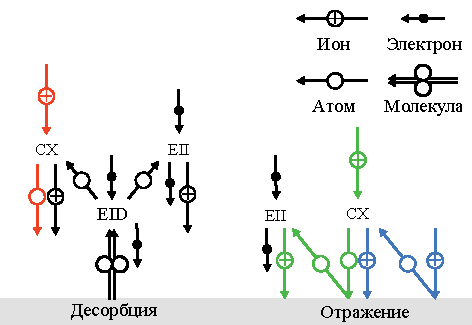
\includegraphics[scale=1.5]{Flux_diagram_simple_rus.pdf}
	}
	\caption{Схематическое представление возможных процессов вблизи поверхности мишени, приводящих к увеличению потока частиц во время ELM-событий: CX "--- резонансная перезарядка, EII "--- ионизация электронным ударом, EID "--- диссоциация электронным ударом}\label{fig:ch3/redeposition}
\end{figure}

Вероятность протекания каждого процесса требует отдельной оценки для конкретных параметров плазмы и приходящих ионов в ходе ELM-событий. Тем не менее, в рамках данной работы проведена оценка влияния перераспределения потока и энергии частиц. Для анализа полагается, что процессы вблизи мишени приводят к изменению потока частиц в \( \beta \) раз с одновременным пропорциональным уменьшением их энергии, поэтому отношение плотности потока частиц к энергии увеличивается на $\beta^2$ при сохранении потока тепла на поверхность. Параметр $\beta$ варьировался в диапазоне от 1 до 10 при тех же условиях, что и в предыдущих расчетах. 

На рисунке~\cref{fig:ch3/beta_var} показаны рассчитанные значения содержания дейтерия в вольфраме после \SI{1000}{\second} комбинированного облучения при разных частотах ELM-событий. 
\begin{figure}[ht]
	\centerfloat{
		\includegraphics[scale=1]{beta_var.pdf}
	}
	\caption{Зависимости интегрального содержания дейтерия в вольфраме после \SI{1000}{\second} облучения при различных значениях отношения плотности потока частиц, приходящих во время ELM-событий, к их энергии. Сплошные линии обозначают средние значения содержания при комбинированном облучении с различными частотами ELM-событий. Верхние границы заштрихованных областей соответствуют \(f_\mathrm{ELM} = \SI{10}{\hertz}\), нижние "--- \(f_\mathrm{ELM} = \SI{100}{\hertz}\). Пунктирные линии показывают зависимости, полученные только при стационарном облучении}\label{fig:ch3/beta_var}
\end{figure}
Увеличение $\beta$ более явно приводит к росту содержания при меньших стационарных нагрузках. Это наблюдается как при фиксированной частоте, так и при фиксированной величине стационарной нагрузки. Можно также заметить, что в случае прихода низкоэнергетичных частиц с большой плотностью потока содержание дейтерия может достигнуть уровня, соответствующего только стационарному облучению. Качественно, повышение скорости накопления дейтерия можно понять из уравнения~\cref{eq:ch3/max_c}: увеличение $\beta$ незначительно повышает произведение $\beta\Gamma (1-r) X(E/\beta)$ ввиду снижения характерной глубины внедрения и увеличения коэффициента отражения. 

\subsection{Влияние параметров центров захвата и скорости рекомбинации на поверхности}

Параметры дефектов определяют вероятности захвата и освобождения атомов дейтерия. Очевидно, что вероятность выхода из дефекта тем больше, чем меньше энергетический барьер для этого. Также ожидается, что материалы с высокой концентрацией дефектов будут характеризоваться большей способностью накапливать дейтерий, чем материалы с идеальной кристаллической структурой. Однако выбор конкретных параметров ловушек для моделирования является открытым вопросом из-за неопределенности, связанной с процессом производства ОПЭ и эволюции дефектов во время облучения.

Упомянутые выше эффекты проиллюстрированы на рисунке~\cref{fig:ch3/eta_Edt_var}, где показаны результаты моделирования при различных значениях концентрации центров захвата и энергетического барьера выхода из них. Во всех сценариях итоговое содержание дейтерия увеличивается с концентрацией дефектов (см. верхний ряд графиков), что согласуется с известными экспериментальными закономерностями. Однако, все еще наблюдается снижение интегрального накопления дейтерия при комбинированном облучении. Причем, разница между значениями растет с концентрацией дефектов.
\begin{figure}[ht]
	\centerfloat{
		\includegraphics[scale=1]{eta_Edt_var.pdf}
	}
	\caption{Зависимости интегрального содержания дейтерия в вольфраме после \SI{1000}{\second} облучения при различных значениях концентрации дефектов (верхний ряд) и барьера выхода из них (нижний ряд). Сплошные линии обозначают средние значения содержания при комбинированном облучении с различными частотами ELM-событий. Верхние границы заштрихованных областей соответствуют \(f_\mathrm{ELM} = \SI{10}{\hertz}\), нижние "--- \(f_\mathrm{ELM} = \SI{100}{\hertz}\). Пунктирные линии показывают зависимости, полученные только при стационарном облучении}\label{fig:ch3/eta_Edt_var}
\end{figure}

Влияние барьера выхода из дефектов на накопление показано в нижнем ряду рисунка~\cref{fig:ch3/eta_Edt_var}. В низкотемпературных режимах (только стационарное облучение при $q_{\mathrm{stat}}=\SI{1}{\mega\watt\per\meter\squared}$) нет никакой разницы между высокоэнергетическими и низкоэнергетическими центрами захвата с точки зрения удержания, поскольку все имплантированные атомы становятся неподвижными. В высокотемпературных режимах содержание увеличивается с барьером освобождения, т.к. большая часть атомов подвижных может оставаться в захваченном состоянии. Поэтому разница между стационарным и комбинированным воздействием нивелируется для случая дефектов с большим барьером освобождения. Значения интегрального содержания могут быть соизмеримы при низких стационарных нагрузках.

Сделанные выводы согласуются с известными закономерностям удержания топлива в ОПЭ, но более важным является увеличение удержания с концентрацией ловушек и барьером освобождения из них. Это предполагает, что образование высокоэнергетичных ловушек в объеме материала во время работы устройства типа ИТЭР (например, из-за нейтронного облучения) может создать условия для повышения скорости накопления изотопов водорода. Это повышение может компенсировать снижение, вызванное дополнительным тепловым потоком, приносимым высокоэнергетическими частицами в течение ELM-событий.

До сих пор представленные расчеты проводились в приближении мгновенной рекомбинации и десорбции на передней поверхности вольфрама. В зависимости от состояния поверхности скорость десорбции может меняться, влияя на динамику удержания изотопов водорода. Для иллюстрации роли рекомбинации на рисунке~\cref{fig:ch3/rec_var} показаны значения содержания дейтерия при различной скорости рекомбинации, варьируемой за счет изменения барьера хемосорбции на поверхности ($E_{\mathrm{c}}$). Для полноты также приведены два частных случая в приближениях мгновенной рекомбинации ($\infty$) и <<чистой>> поверхности ($E_{\mathrm{c}}=0$).

\begin{figure}[ht]
	\centerfloat{
		\includegraphics[scale=1]{rec_var.pdf}
	}
	\caption{Зависимости интегрального содержания дейтерия в вольфраме после \SI{1000}{\second} облучения при различных значениях скорости рекомбинации на поверхности. Сплошные линии обозначают средние значения содержания при комбинированном облучении с различными частотами ELM-событий. Верхние границы заштрихованных областей соответствуют \(f_\mathrm{ELM} = \SI{10}{\hertz}\), нижние "--- \(f_\mathrm{ELM} = \SI{100}{\hertz}\). Пунктирные линии показывают зависимости, полученные только при стационарном облучении}\label{fig:ch3/rec_var}
\end{figure}

Согласно данным, приближение мгновенной рекомбинации воспроизводит результаты, полученные при низких значениях барьера хемосорбции. Увеличение барьера хемосорбции снижает скорость рекомбинации на поверхности, что приводит к росту скорости накопления дейтерия. Это увеличение более явно наблюдается в случае комбинированного воздействия, поскольку используемый коэффициент рекомбинации Пика и Сонненберга уменьшается с температурой. Анализируя данные для наибольшего значения барьера хемосорбции, можно также заметить, что результаты при комбинированном воздействии близки к полученным без учета ELM-событий. Это также позволяет предположить возможное повышение скорости накопления дейтерия в случае образования на поверхности потенциального барьера, например, из-за примесных атомов.

\subsection{Эффективность обезгаживания}

Все приведенные результаты указывают на снижение скорости накопления при наступлении ELM-событий. В то же время нагрев до более высоких температур относительно базовых нагрузок приводит к миграции дейтерия в объем, где он накапливается в дефектах. Помимо того, что ускоренная диффузия может влиять на время проникновения в систему охлаждения, она также может усложнять процесс удаления трития. В ИТЭР в качестве базовых механизмов для этого рассматриваются изотопный обмен и прогрев ОПЭ, причем второй подход предполагается использовать для обезгаживания толстых поверхностных слоев (в т.ч. соосажденных слоев). Во время длительных этапов обслуживания планируется осуществлять нагрев ОПЭ за счет пропускания горячей воды под давлением через систему охлаждения моноблоков. При таком подходе возможно достижение температуры ОПЭ в \SI{513}{\kelvin}~\cite{Pitts2025}.

Для оценки влияния появления ELM-событий на эффективность последующего обезгаживания ОПЭ была проведена дополнительная серия расчетов. Рассматривалось три этапа: облучение длительностью \SI{100}{\second}; простой и охлаждение материала длительностью \SI{1}{\hour}; обезгаживание материала при постоянной температуре \SI{513}{\kelvin} длительностью \SI{25}{\day}. Рассматривался один тип центров захвата с концентрацией \SI{e-2}{\text{ат.}\percent} и барьером освобождения \SI{1}{\electronvolt}. 

Пример полученных временных зависимостей температуры поверхности и содержания дейтерия в вольфраме приведен на рисунке~\cref{fig:ch3/baking_single} для двух случаев облучения: при учете влияния ELM-событий и без.
\begin{figure}[ht]
	\centerfloat{
		\includegraphics[scale=1]{baking_single.pdf}
	}
	\caption{Временные зависимости температуры поверхности (вверху), содержания дейтерия (по середине) и содержания дейтерия, нормированного на значение в начале процедуры обезгаживания для двух случаев облучения при \(q_\mathrm{stat}= \SI{5}{\mega\watt\per\meter\squared}\)}\label{fig:ch3/baking_single}
\end{figure}
В случае только стационарного облучения содержание существенно превышает достигаемое значение при ELM-событиях. После начала процедуры обезгаживания в обоих случаях наблюдается уменьшение количества захваченных атомов, однако зависимость в случае ELM-событий спадает более плавно, что напрямую связано с пространственным распределением захваченного дейтерия на момент начала процедуры.

Расчетная эффективность обезгаживания (интегральное число десорбированных частиц отнесенное к их начальному количеству) для всех сценариев облучения приведена на рисунке~\cref{fig:ch3/baking_efficiency}.
\begin{figure}[ht]
	\centerfloat{
		\includegraphics[scale=1]{baking_efficiency.pdf}
	}
	\caption{Зависимость эффективности обезгаживания от частоты ELM-событий в трех модельных сценариях облучения. Значения при нулевой частоте соответствуют случаю облучения только стационарными потоками тепла и частиц}\label{fig:ch3/baking_efficiency}
\end{figure}
Из рисунка видно, что наибольшая эффективность достигается в случае только стационарного облучения. С увеличением фоновой нагрузки и частоты ELM-событий эффективность уменьшается, что вызвано проникновением дейтерия на большую глубину при нагреве материала до более высоких температур. Можно также заметить, что при высоких частотах эффективность обезгаживания в самом <<горячем>> сценарии немного увеличивается. Это вызвано достижением атомами дейтерия правой границы расчетной области за рассмотренное время процедуры. Таким образом, проведенное моделирование явно демонстрирует, что протекание переходных процессов может влиять как на скорость накопления дейтерия во время плазменных разрядов, так и на эволюцию его содержания в ОПЭ во время иных этапов эксплуатации установки. 

\section{Аналитический анализ}\label{sec:ch3/sec3}

В предыдущем разделе были представлены результаты моделирования, ограниченного случаем \SI{1000}{\second} непрерывного облучения во время ELM-событий. Ввиду необходимости использования малого временного шага интегрирования расчеты такого типа оказываются более времязатратными, чем в случае моделирования накопления изотопов водорода при стационарном облучении. Время расчета на одном ядре процессора Intel Xeon Gold 6240 достигало \SI{72}{\hour} в случае непрерывного облучения при частоте ELM-событий равной \SI{100}{\hertz}. Данное время является приемлемым, но указывает на то, что решение аналогичной задачи в трехмерной геометрии на временных масштабах, соизмеримых со сроком службы установки (\( \sim \SI{e6}{\second}\)), потребует гораздо больших временных и вычислительных ресурсов. В аналогичном исследовании~\cite{Dasgupta2023} рассматривался захват дейтерия под действием импульсно-периодических тепловых нагрузок при стационарном потоке частиц и без учета влияния дефектов. В работе было предложено использовать осредненный по длительности ELM-события тепловой поток для упрощения моделирования и снижения вычислительных затрат. В этом разделе проведен анализ применимости подхода к решению полной задачи транспорта дейтерия в вольфраме.

\subsection{Квазистационарное приближение}
Переход к осредненным величинам (т.н. осреднение по Рейнольдсу) подразумевает разделение периодических потоков тепла и частиц на медленно меняющиеся и флуктуирующие части~\cite{Marenkov2012a}:
\begin{subequations}
	\label{eq:ch3/periodic_funcs}
	\begin{align}
		q_{\mathrm{ELM}}(t)&=\overline{q}_{\mathrm{ELM}} + \widetilde{q}_{\mathrm{ELM}}(t),\label{eq:decomp_heat}\\
		\Gamma_{\mathrm{ELM}}(t)&=\overline{\Gamma}_{\mathrm{ELM}} + \widetilde{\Gamma}_{\mathrm{ELM}}(t),
	\end{align}
\end{subequations}
где $\overline{q}_{\mathrm{ELM}}$ ($\overline{\Gamma}_{\mathrm{ELM}}$) "--- средний по времени поток тепла (частиц), приходящий за период ELM-события. Средние значения легко получить путем интегрирования выражений~\cref{eq:ch3/elm_fluxes}:
\begin{subequations}
	\label{eq:ch3/av_funcs}
	\begin{align}
		\overline{q}_{\mathrm{ELM}}&=f_{\mathrm{ELM}}\varepsilon_\parallel\sin(\alpha)\label{eq:av_heat},\\
		\overline{\Gamma}_{\mathrm{ELM}}& =\frac{\sqrt{\pi}}{2} \Gamma_{0,\mathrm{ELM}}\,\xi\,\mathrm{erfc}\left(\xi\right),\label{eq:av_flux}
	\end{align}
\end{subequations}
где $\xi=\tau f_{\mathrm{ELM}}$, $\mathrm{erfc(x)}$ "--- дополнительная функция ошибок.

Подстановка разложенного теплового потока в уравнение теплопроводности позволяет отдельно проанализировать поле средней температуры. Несмотря на то, что тепловые свойства материала зависят от температуры нелинейно, вклад их изменения в эволюцию средней температуры материала будет небольшим. Индуцированное повышение температуры из-за поверхностного теплового импульса пропорционально $1/\sqrt{\kappa C \rho}$, которое медленно меняется с температурой. С другой стороны, полное аналитическое рассмотрение реакционно-диффузионной задачи гораздо сложнее, учитывая экспоненциальную зависимость констант скорости процессов от температуры.

\begin{comment}
	 В случае переноса тепла требуем: \( \underset{t}{\max} \, |\widetilde{q}_{\mathrm{ELM}}| \ll \overline{q}_{\mathrm{tot}} \), где \( \overline{q}_{\mathrm{tot}} = q_\mathrm{stat} + \overline{q}_{\mathrm{ELM}} \). Для задачи транспорта дейтерия необходимо, чтобы амплитуда изменения флуктуирующей части объемного источника атомов была мала: \( \underset{t}{\max} \, |\widetilde{S}_{\mathrm{ELM}}| \ll \overline{S}_{\mathrm{tot}} \), где \( \overline{S}_{\mathrm{tot}} = S_\mathrm{stat} + \overline{S}_{\mathrm{ELM}} \).
\end{comment}

Основной интерес в вопросе длительного накопления изотопов водорода в ОПЭ представляет среднее значение содержания, которое будет сохраняться по окончании плазменного разряда. Провести аналитический анализ можно в приближении малых ELM-вспышек~\cite{Marenkov2012a}, когда амплитуды флуктуирующих компонент потоков малы по сравнению со средними. В данном приближении эволюция концентрации атомов будет определяться средними компонентами вплоть до достижения квазистационарного режима. В случае больших ELM-вспышек, члены, связанные с флуктуациями, будут влиять на изменение средних компонент. Чтобы различить эти два случая, можно сравнить средние и флуктуирующие компоненты температуры и объемного источника атомов в задаче транспорта дейтерия.

Пренебрегая охлаждением за счет излучения, подстановка компонент потока тепла с последующим осреднением уравнения теплопроводности по длительности ELM-события позволяет легко получить квазистационарное распределение температуры:
\begin{equation}
	\label{eq:ch3/temp_av}
	\overline{T}(x)=T_\mathrm{r}+\overline{q}_{\mathrm{tot}}\,\int\limits_x^L\frac{dx}{\kappa(\overline{T})},
\end{equation}
где, $T_\mathrm{r}$ "--- равновесная температура на задней границе материала, которая находится из баланса теплового потока: $\overline{q}_{\mathrm{tot}}=q_{\mathrm{loss}}^*(T_\mathrm{r})$ (см. уравнение~\cref{eq:ch3/heat_WCu}). Максимальное колебание температуры из-за потока тепла на границе можно оценить как:
\begin{equation}
	\label{eq:ch3/temp_fluct}
	\widetilde{T}^{\max} \propto \widetilde{q}_{\mathrm{ELM}}^{\max} \sqrt{\frac{\tau}{\kappa C \rho}}.
\end{equation} 

Вычислив значение среднего теплового потока, можно заметить, что $\widetilde{q}_{\mathrm{ELM}}^{\max} \approx q_{\mathrm{ELM}}^{\max}$. Тепловой поток во время ELM-события достигает максимального значения $q_{\mathrm{ELM}}^{\max}\approx 0.84 \, q_{0,\mathrm{ELM}}$ при $\tau/t\approx 1.27$. Индуцированное колебание температуры можно считать малым, если $\widetilde{T}^{\max} \ll \overline{T}(x=0)$. Оценку можно получить, полагая, что свойства материала не зависят от температуры:
\begin{equation}
	\label{eq:heat_condition}
	q_{0,\mathrm{ELM}} \ll \overline{q}_{\mathrm{tot}}\,\frac{ L}{L_{\mathrm{heat}}}\,\left( 1+\frac{T_\mathrm{r}\kappa}{\overline{q}_{\mathrm{tot}}L}\right),
\end{equation}
где $L_{\mathrm{heat}}=\sqrt{\kappa\tau/C\rho}$ "--- характерная глубина распространения тепла за время длительности ELM-события. Для объемных источников атомов справедливо аналогичное соотношение: $\widetilde{S}^{\max}_{\mathrm{ELM}} \ll \overline{S}_{\mathrm{tot}}$, где $\overline{S}_{\mathrm{tot}}=S_{\mathrm{stat}}+\overline{S}_{\mathrm{ELM}}$. Аналогично предыдущему случаю, максимальная амплитуда флуктуации потока частиц из-за ELM-вспышки приблизительно равна: $\widetilde{\Gamma}_{\mathrm{ELM}}^{\max} \approx \Gamma_{\mathrm{ELM}}^{\max}$. Поток частиц достигает максимума при $t=\tau$ со значением $\Gamma_{0,\mathrm{ELM}}/\exp(1)$. Обобщая начальное соотношение и используя параметры пространственного распределения источников, можно прийти к следующему условию:
\begin{equation}
	\label{eq:flux_condition}
	\Gamma_{0,\mathrm{ELM}} \ll \Gamma_{\mathrm{stat}}\,\frac{\varphi_{\mathrm{stat}}(X_\mathrm{stat})(1-r_{\mathrm{stat}})}{\varphi_{\mathrm{ELM}}(X_\mathrm{ELM})(1-r_{\mathrm{ELM}})}.
\end{equation}
Оба соотношения наглядно демонстрируют требование малости амплитуд осциллирующих компонент потоков во время ELM-событий. Исходя из предыдущего раздела, такие условия могут быть достигнуты при высоких частотах ELM-событий. Стоит заметить, что соотношения не являются независимыми, поскольку поток тепла зависит от потока частиц.

Для демонстрации применимости подхода на рисунке~\cref{fig:ch3/Eqv_load} приведено сравнение временных зависимостей содержания дейтерия, полученных двумя способами: путем моделирования накопления под действием обеих компонент потоков и с помощью только средних потоков. В соответствии с приведенным выше анализом отклонение результатов, полученных со средними компонентами потоков, уменьшается при более высоких частотах ELM-событий и фоновых нагрузках. В случае $q_{\mathrm{stat}}=\SI{10}{\mega\watt\per\meter\squared}$ результаты хорошо согласуются во всем диапазоне ELM-частот. Использование средних компонент потоков существенно снижает время вычислений (с дней до минут), что может быть использовано при проведении комплексных оценок накопления изотопов водорода во всей первой стенке ИТЭР.

\begin{figure}[ht]
	\centerfloat{
		\includegraphics[scale=1]{Eqv_load.pdf}
	}
	\caption{Сравнение временных зависимостей содержания дейтерия, полученных при моделировании с учетом обеих компонент потоков тепла и частиц (сплошные линии) и с учетом только средних компонент (пунктирные линии)}\label{fig:ch3/Eqv_load}
\end{figure}

\subsection{Распределение концентрации дейтерия при насыщении}\label{sec:ch3/sec3/subsec2}
Использование средних компонент нагрузок позволяет получить аналитические выражения для распределения концентрации дейтерия при насыщении с учетом влияния градиента температуры, что является обобщением выражений, полученных ранее~\cite{Denis2022}. Рассмотрим стационарную форму задачи транспорта~\cref{eq:ch2/mobile_conc}, полагая что источники подвижных атомов являются точечными и каждый из них расположен на характерной глубине внедрения:
\begin{subequations}
	\label{eq:ch3/eq:solute_analytic}
	\begin{gather}
	\frac{\partial}{\partial x}\left(D(\overline{T})\left[\frac{\partial \overline{c}_{\mathrm{m}}}{\partial x} +H(\overline{T})\overline{c}_{\mathrm{m}}\right] \right)= - S_{\mathrm{stat}}^{\delta}-\overline{S}_{\mathrm{ELM}}^{\delta}, \label{eq:ch3/solute_analytic}\\
	\overline{c}_{\mathrm{t}}=\dfrac{n_{\mathrm{t}}}{1+\dfrac{n_{\mathrm{t}}\nu_{\mathrm{dt}}(\overline{T})}{\overline{c}_{\mathrm{m}}\nu_{\mathrm{t}}(\overline{T})}},\label{eq:ch3/trapped_analytic}
	\end{gather}
\end{subequations}
где $S_i^\delta=\Gamma_i^{\mathrm{imp}}\delta(x-X_i)$; $\delta(x)$ "--- дельта-функция Дирака; $H(\overline{T})=Q(\overline{T})\partial_x \overline{T}/k\overline{T}^2$. Стоит заметить, что уравнение~\cref{eq:ch3/trapped_analytic} можно обобщить на случай нескольких типов центров захвата, имеющих неравномерное пространственное распределение. Однако мы ограничимся случаем одного центра захвата, рассмотренного в работе. Решение уравнения~\cref{eq:ch3/solute_analytic} можно получить для однородного граничного условия Дирихле на облучаемой поверхности и условия Дирихле или Неймана на обратной поверхности.

Решение стационарного уравнения транспорта проводится методом функции Грина с применением теоремы о суперпозиции (см. приложение~\cref{app:E}). Для используемой в работе теплоты переноса ($Q(T)=-0,0045\,kT^2$), параметр $H$ не зависит от температуры. Таким образом, решение ур.~\cref{eq:ch3/solute_analytic}:
\begin{subequations}
	\begin{gather}
	\label{eq:ss_solution}
	\begin{array}{ll}
		\overline{c}_{\mathrm{m}}=&\exp\left(-Hx\right)\times
			\begin{cases}
			C_1(x,X_{\mathrm{stat}})+C_1(x,X_{\mathrm{ELM}}), & x \in [0,X_{\mathrm{stat}}],\\
			C_2(x,X_{\mathrm{stat}})+C_1(x,X_{\mathrm{ELM}}), & x \in [X_{\mathrm{stat}},X_{\mathrm{ELM}}],\\
			C_2(x,X_{\mathrm{stat}})+C_2(x,X_{\mathrm{ELM}}), & x\in [X_{\mathrm{ELM}}, L],
			\end{cases}
	\end{array}\\
	C_1(x,X_i)=\Gamma_i^{\mathrm{imp}}G_1(x,X_i),\\
	C_2(x,X_i)=\Gamma_i^{\mathrm{imp}}G_2(x,X_i),
	\end{gather}
\end{subequations}
где функция Грина определяется с помощью уравнений~\cref{eq:Green_solution_D} для случая граничного условия Дирихле на правой поверхности и с помощью уравнений~\cref{eq:Green_solution_N} для случая граничного условия Неймана. Данные выражения позволяют построить распределение концентрации дейтерия с учетом решения стационарного уравнения теплопроводности.

На рисунке~\cref{fig:ch3/retention_saturation} показано сравнение аналитических профилей концентрации с рассчитанными численно для трех различных случаев:
\begin{enumerate}[beginpenalty=10000]
	\item $q_{\mathrm{stat}}=\SI{1}{\mega\watt\per\meter\squared}$, $f_{\mathrm{ELM}}=\SI{10}{\hertz}$, $n_{\mathrm{t}}=\SI{e-3}{\text{ат.}\percent}$;
	\item $q_{\mathrm{stat}}=\SI{5}{\mega\watt\per\meter\squared}$, $f_{\mathrm{ELM}}=\SI{50}{\hertz}$, $n_{\mathrm{t}}=\SI{e-2}{\text{ат.}\percent}$;
	\item $q_{\mathrm{stat}}=\SI{10}{\mega\watt\per\meter\squared}$, $f_{\mathrm{ELM}}=\SI{100}{\hertz}$, $n_{\mathrm{t}}=\SI{e-2}{\text{ат.}\percent}$.	
\end{enumerate}
В расчетах барьер выхода из дефектов был равен \SI{1}{\electronvolt}. Расчетные профили концентрации при средних компонентах нагрузок были получены с гауссовым распределением источников внедренных атомов. Моделирование проводилось до достижения насыщения. Для иллюстрации, содержание дейтерия достигает 99\% от стационарного уровня за время $\approx\SI{16300}{\second}$ во втором модельном случае с граничным условием Дирихле, заданным на обеих границах. Распределения концентрации, полученные с помощью обоих подходов, демонстрируют, что доминирующая часть атомов захватывается в холодной области вблизи правой границы. Аналитические профили хорошо коррелируют с полученными на основе численного расчета профилями при различных комбинациях входных параметров, но представляют собой незначительно заниженную оценку, т.к. не учитывают протяженность профиля внедренных частиц. 

\begin{figure}[ht]
	\centerfloat{
		\includegraphics[scale=1]{retention_saturation.pdf}
	}
	\caption{Сравнение аналитических профилей концентрации дейтерия при насыщении (тонкие линии) с профилями, полученными на основе численных расчетов с использованием средних компонент потоков тепла и частиц (широкие линии)}\label{fig:ch3/retention_saturation}
\end{figure}


\section{Выводы к главе 3}
Проведено численное моделирование динамики захвата дейтерия в вольфрамовых элементах под действием импульсных плазменных нагрузок. Применимость использованной модели продемонстрирована путем воспроизведения результатов ТДС-измерений после импульсного облучения на установке КСПУ-Т. Получено согласие между моделированием и экспериментом при предположении ограниченной скорости десорбции с поверхности.   

Результаты численных расчетов по длительному облучению поверхности вольфрама в условиях, релевантных ELM-событиям в ИТЭР, указывают на снижение скорости накопления в широком диапазоне параметров. Снижение вызвано дополнительным нагревом до более высоких температур из-за прихода высокоэнергетичных частиц с плотностью потока, соизмеримой со случаем стационарного облучения. В рамках представленного подхода это снижение более явно проявляется с ростом частоты ELM-событий при меньших базовых нагрузках. Было выявлено несколько факторов (ограниченная скорость десорбции, наличие центров захвата с большим барьером освобождения), способных повысить скорость накопления во время ELM-событий. С другой стороны, нагрев материала до высоких температур во время переходных процессов обеспечивает условия для более быстрой диффузии в объем. Повышенная подвижность может влиять на время проникновения изотопов водорода (в т.ч. трития) в систему охлаждения ОПЭ и на эффективность последующего обезгаживания между экспериментальными кампаниями. В силу этого, ранние оценки содержания при базовых сценариях разрядов в ИТЭР без учета влияния ELM-событий могут быть завышенными. 

В приближении малых амплитуд импульсных нагрузок во время ELM-событий продемонстрирована применимость использования только средних компонент для получения оценок содержания. Использование средних компонент нагрузок радикально снижает сложность вычислений и позволяет быстро оценить уровень накопления при небольших ELM-вспышках. В рамках подхода также были получены аналитические выражения, определяющие распределения дейтерия в приближении точечных источников подвижных атомов при наличии центров захвата и градиента температуры. Аналитические выражения хорошо согласуются с результатами численных расчетов и могут быть использованы для оценки содержания дейтерия при насыщении.

\clearpage
